%%%%%%%%%%%%%%%%%%%%%%%%%%%%%%%%%%%%%%%%%%%%%%%%%%%%%%%%%%%%%%%%%%%
%%% Documento LaTeX 																						%%%
%%%%%%%%%%%%%%%%%%%%%%%%%%%%%%%%%%%%%%%%%%%%%%%%%%%%%%%%%%%%%%%%%%%
% Título:		Capítulo 1
% Autor:  	Ignacio Moreno Doblas
% Fecha:  	2014-02-01, actualizado 2019-11-11
% Versión:	0.5.0
%%%%%%%%%%%%%%%%%%%%%%%%%%%%%%%%%%%%%%%%%%%%%%%%%%%%%%%%%%%%%%%%%%%
% !TEX root = A0.MiTFG.tex
\chapterbegin{Tecnología empleada}

\label{chp:ManLaTeX}
\minitoc
\vspace{1cm}
En este apartado se van a explicar las plataformas o elementos, tanto hardware como 
software, sobre los que se ha desarrollado este proyecto. 

\section{Plataforma hardware}
El sistema hardware empleado va a ser un dispositivo FPGA. Una matriz de puertas lógicas 
programables (FPGA) se define como un dispositivo electrónico programable que contiene 
bloques de lógica cuya interconexión y funcionalidad puede ser configurada en el momento, 
mediante un lenguaje de descripción especializado. La lógica programable puede reproducir 
desde funciones tan sencillas como las llevadas a cabo por una puerta lógica o un sistema 
combinacional hasta complejos sistemas en un chip. Su principal 
ventaja es que pueden ser reprogramados para un trabajo específico o cambiar sus 
requisitos después de haberse fabricado. El inventor de esta tecnología fue 
Xilinx. \cite{fpga}

La principal característica es la flexibilidad. Esto también implica que en muchos
casos se pueden hacer cambios físicos sin hacer modificaciones costosas en la placa.

La segunda característica es la aceleración. 
Estos dispositivos son muy fáciles de fabricar y se venden preparados para ser usados 
directamente, lo cual conlleva una disminución en los tiempos durante el 
proceso de producción. 
En el apartado de diseño, una FPGA está lista en cuanto su diseño inicial esté finalizado
y testeado, lo cual, de nuevo, ahorra tiempo. Finalmente, para la aceleración, las FPGA, 
mediante aceleraciones de carga y descarga de información, aumentan el 
rendimiento global del sistema. \cite{fpga}

Normalmente la programación de los FPGA se realiza en lenguajes de 
bajo nivel llamados Verilog o VHDL. Ambos son similares y sirven para 'describir' cómo
la FPGA debe manejar el hardware del mismo. Esto se desarrollará con mayor profundidad
y detalle en el apartado software (2.2).

Para el desarrollo de este trabajo se ha elegido como FPGA la Red Pitaya STEMlab 125-14 
que se describe a continuación.

\subsection{Red Pitaya}

La elección de la FPGA es una fase muy importante ya que será la base del 
desarrollo de todo el proyecto, por lo tanto, se van a detallar sus características 
más representativas, así como sus ventajas e inconvenientes.

La figura \ref{pitaya} presenta la Red Pitaya cuyas características se especifican 
seguidamente.

\begin{figure}[ht]
    \centering
    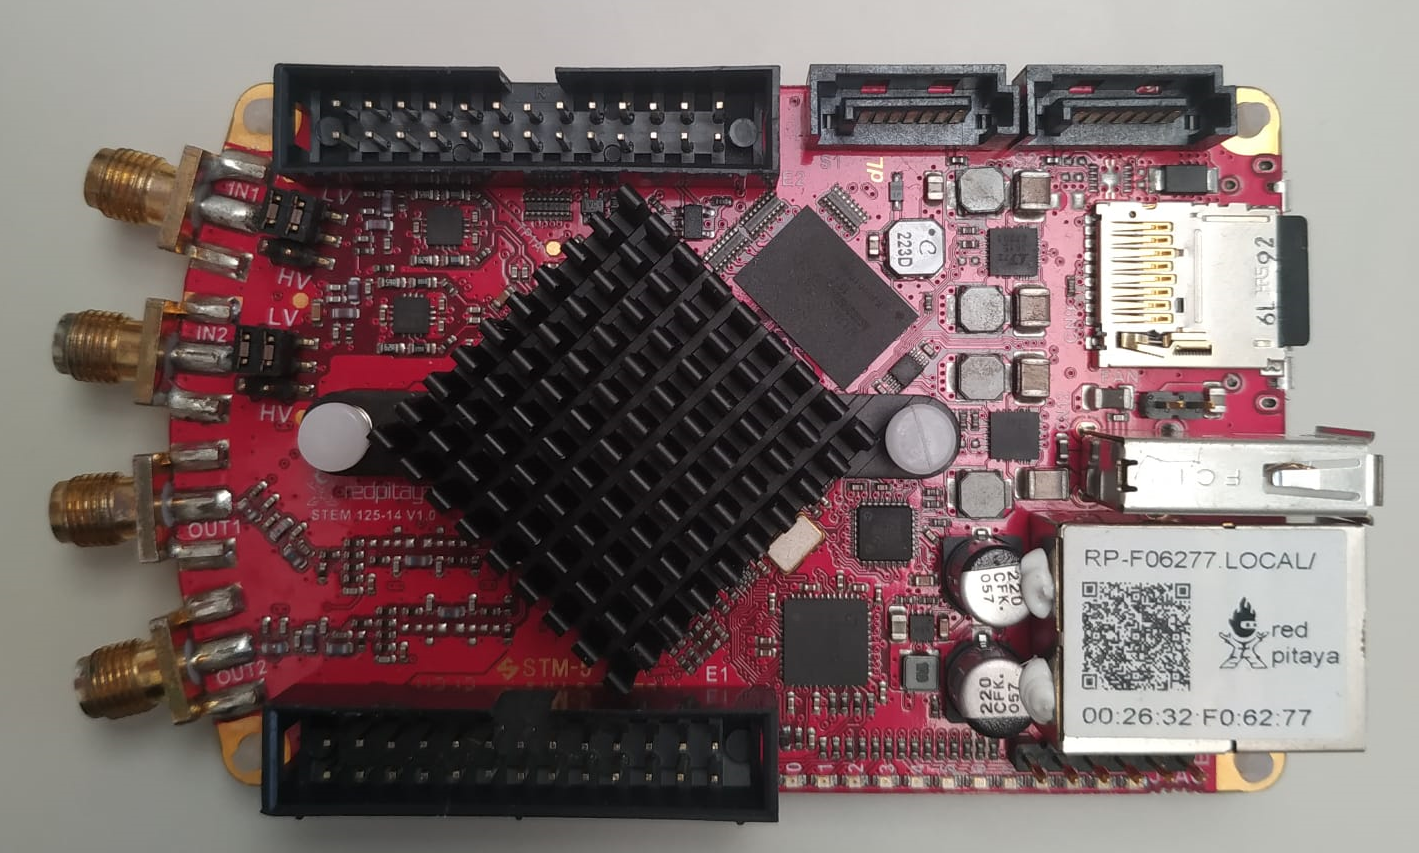
\includegraphics[scale=0.25]{./figuras/pitaya.png}
    \caption{\small{Red Pitaya.}}
    \label{pitaya}%
\end{figure}

Red Pitaya es un sistema electrónico \textit{'open source'} o de código abierto 
desarrollado por \textit{Instrumentation Technologies} para
aplicaciones de control y medición con un tamaño relativamente pequeño. Los dos 
principales factores diferenciales y los que más nos interesan son 
su hardware dedicado para la adquisición y generación de señales analógicas y
su CPU programable para realizar tareas de procesamiento digital
de señales. 

La figura \ref{com_pitaya} muestra, en detalle, los elementos que forman la Red Pitaya.
De todos los que se aprecian en la imagen los que más nos importan son la conexión de 
alimentación, la conexión Ethernet, con la cual nos comunicaremos con la Red Pitaya,
los pines de entrada y salida para transmitir y/o recibir la señal, la memoria RAM y
el procesador más FPGA.

\begin{figure}[ht]
    \centering
    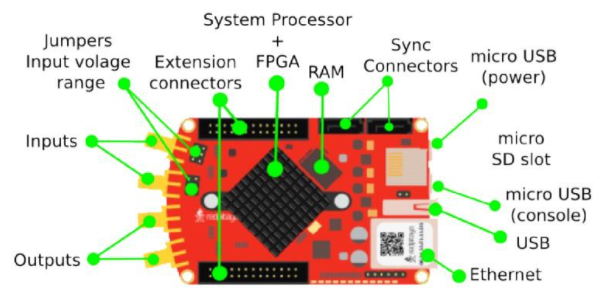
\includegraphics[scale=0.80]{./figuras/comp_pitaya.png}
    \caption{\small{Componentes Red Pitaya. Fuente[8]}}
    \label{com_pitaya}%
\end{figure}

Especificaciones básicas: \cite{pitaya}
\begin{itemize}
    \item Procesador: Dual Core ARM Cortex A9.
    \item FPGA: Xilinx Zynq 7010.
    \item RAM: 512 MB (4Gb).
    \item Consumo: 1,5A.
    \item Conexión de alimentación: Micro USB.
    \item Conectividad: Ethernet.
    \item USB 2.0
    \item Sistema operativo: Linux.
\end{itemize}

Además de las especificaciones nombradas anteriormente, las fundamentales para este 
proyecto son las relacionadas con las entradas y salidas ya que serán las encargadas
de transmitir la señal al transceptor óptico y de interpretar la señal recibida por 
el receptor óptico. La Red Pitaya tiene dos pines de entrada con una resolución del 
ADC de 14 bits y con un rango de tensión de ±1V que nos permite usar toda la resolución
ya que son los niveles de tensión que nos proporciona el receptor óptico. Para la 
transmisión cuenta con dos pines de salida con una resolución del DAC de 14 bits. \cite{pitaya}


\section{Plataforma software}
% [Hablar sobre la plataforma sobre la que se ha programado la fpga (vivado) comentando sus 
% características y sus principales funciones y en que aplicaciones es recomendable su uso.
% Hablar sobre que el programa en c que es el que ejecuta las transmisiones y recepciones 
% y es el encargado de poner en
% funcionamiento el enlace además de comprobar los paquetes, etc.]
En esta sección se va a describir el apartado software con el que se ha implementado
y desarrollado el proyecto. Consta de dos puntos diferenciales que son la 
programación de la FPGA y la programación en C encargada de generar la trama y de 
controlar la recepción de la misma.

La programación de la FPGA se ha realizado en el entorno Vivado. Vivado Design Suite
es un paquete de software producido por Xilinx para la síntesis y análisis de diseños 
HDL, reemplazando a Xilinx ISE con características adicionales para el desarrollo de 
sistemas en un chip y síntesis de alto nivel. 

Vivado se creó en 2012 y es un entorno de diseño integrado (IDE) que ofrece un ámbito
de desarrollo de próxima generación con orientación SoC (\textit{System on Chip}), 
centrado en IP,
que se ha creado desde cero para mejorar la productividad en la integración e 
implementación de los sistemas. \cite{vivado}

Vivado es compatible con los dispositivos de las siguientes familias: UltraScale, 
Virtex-7, Kintex-7, Artix-7 y Zynq-7000. Como se ha visto en el apartado anterior la 
Red Pitaya tiene Zynq-7000 por lo que son perfectamente compatibles. Además, el 
compilador de Vivado permite que los programas en C se dirijan directamente a los 
dispositivos sin la necesidad de crear manualmente un RTL, lo que implica una gran 
ventaja para el funcionamiento global del sistema. \cite{vivado}

Una de las mayores ventajas de este programa es la facilidad del uso y de la creación
de diagramas de bloques lo que supone un desarrollo más lineal e intuitivo. 

A continuación, en la figura \ref{vivado}
se muestra una imagen del interfaz de Vivado sobre el que se ha 
trabajado e implementado el proyecto.

\begin{figure}[ht]
    \centering
    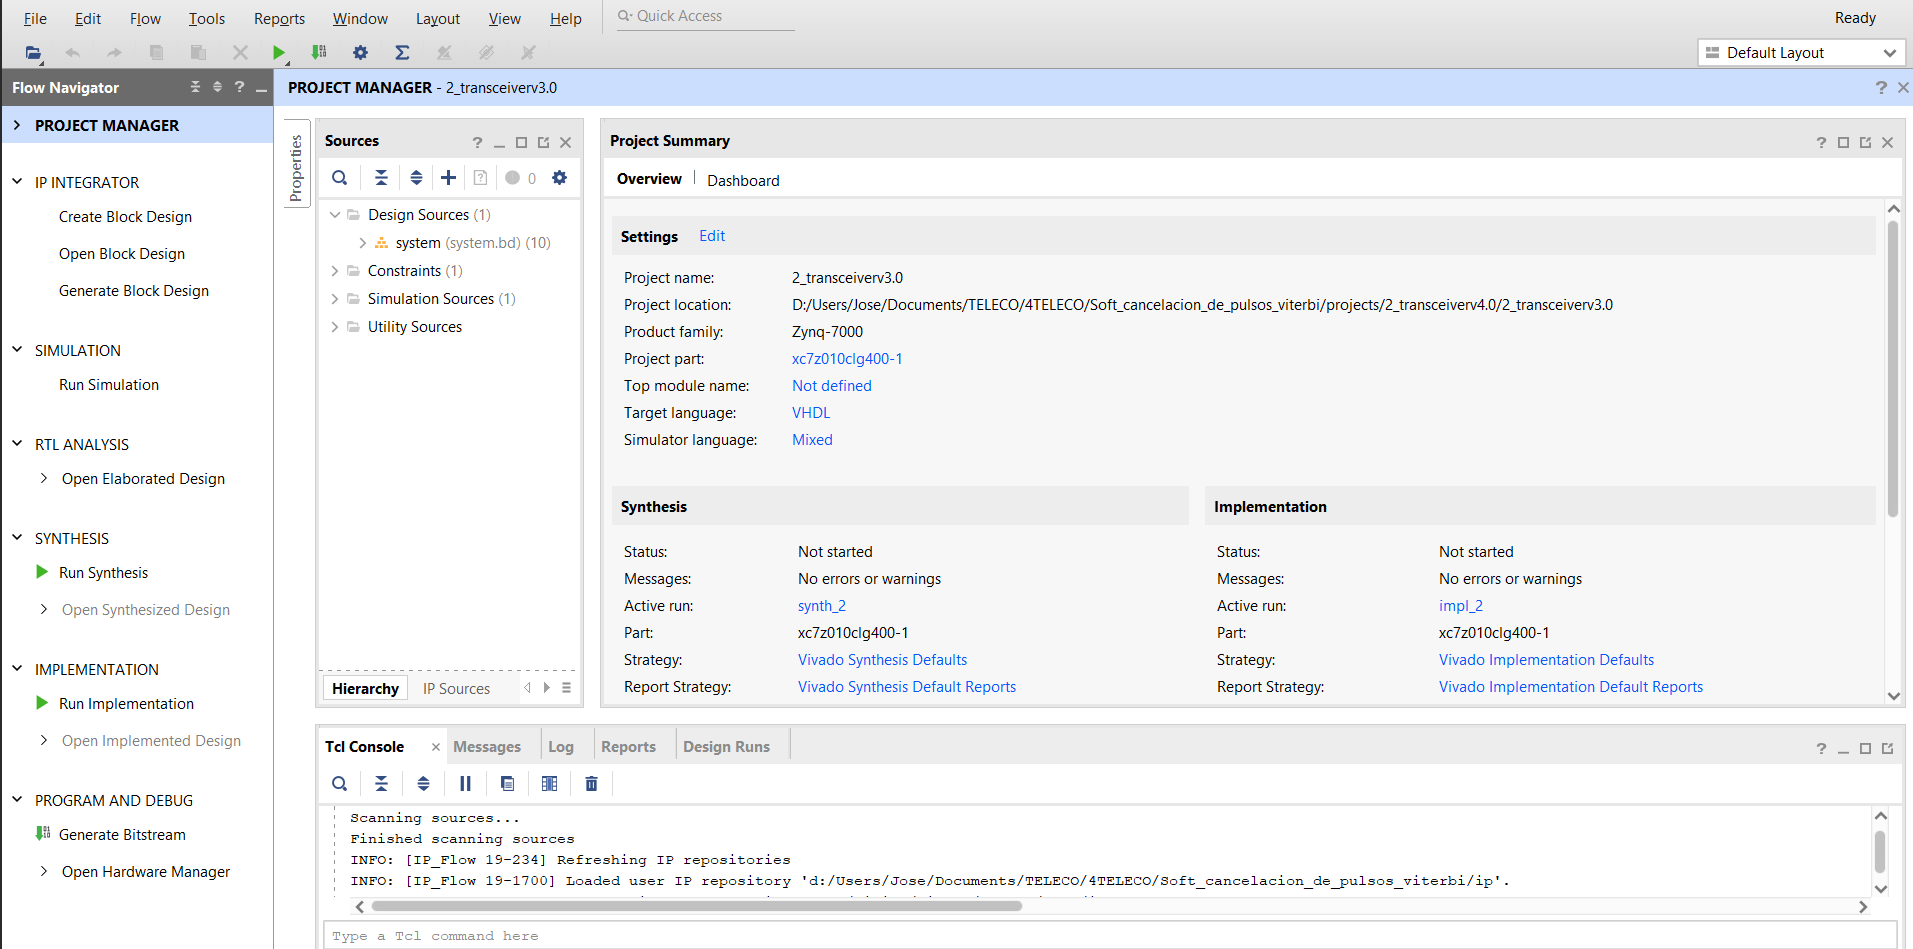
\includegraphics[scale=0.37]{./figuras/vivadoo.png}
    \caption{\small{Interfaz del programa Vivado.}}
    \label{vivado}%
\end{figure}
\newpage
Por todo lo comentado anteriormente se ha considerado que Vivado es la herramienta 
ideal para la programación de la Red Pitaya siendo la encargada de la implementación del 
proyecto. 

El programa en C es la denominada aplicación funcional para realizar la transmisión y 
recepción de la trama mediante el enlace de luz con el hardware programado a través
de Vivado.

Esta aplicación funcional se ha desarrollado para hacer pruebas sobre el transceptor 
hardware de una forma sencilla, tanto en una misma Red Pitaya, como usando una como 
transmisor y otra como receptor. Su funcionalidad general es transmitir 1000 paquetes 
(modificable en el programa en C) y recibirlos a través de dicho programa en C desde 
el terminal, pudiendo identificar paquetes erróneos,
correctos y perdidos. También se puede elegir el esquema de señalización con el que se 
quiere transmitir (pulsos alternos, cancelación de pulsos y 4PPM) y el sistema de decisión
con el cual se quiere interpretar la señal recibida (\textit{hard-decoding}, 
\textit{soft-decoding} o Viterbi).

También es dinámica la forma en la que se elige la frecuencia, pudiendo 
introducirla en el comando de ejecución usando el mismo bitstream para todo el rango de 
frecuencia (100kHz - 4.8MHz).

Para compilar la aplicación se ejecuta el programa make que compila los ficheros aunque
en el anexo Manual de utilización de la aplicación se explica todo el proceso de ejecución
más detalladamente.

\chapterend{}